% !TEX root = ../sma-kirigami-icems-2021.tex
\documentclass[border=1mm,
               class=article
               preview]{standalone}
\usepackage{tikz}
% trim={<left> <lower> <right> <upper>}
\begin{document}
\begin{tikzpicture}
    \node[anchor=south west,inner sep=0] (graph) at (0,0) {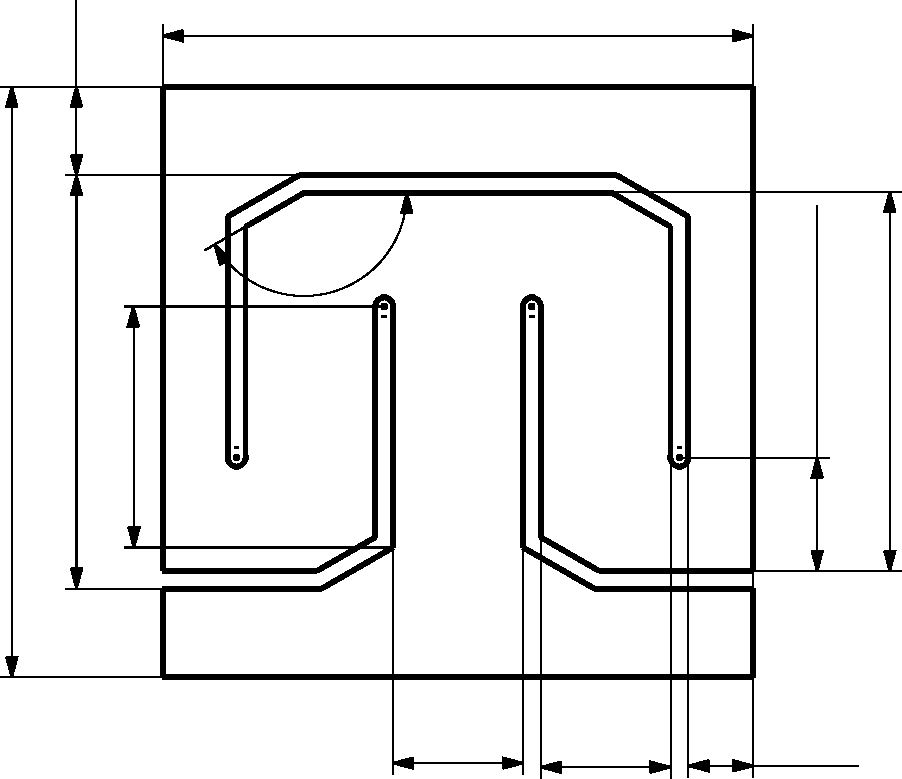
\includegraphics[width=0.5\textwidth]{images/chap5/kirigami-parametrisation.pdf}};
    \begin{scope}[x={(graph.south east)},y={(graph.north west)}]
      \node (phi) at (0.37,0.67) {$\phi$};
      \node (wout0) at (0.51,-0.02) {$w$};
      \node (wout1) at (0.68,-0.02) {$w$};
      \node (wout2) at (0.92,0.06) {$w/2$};
      \node[rotate=90] (l) at (-0.02,0.5) {$L$};
      \node[rotate=90] (l) at (0.055,0.5) {$\alpha L$};
      \node[rotate=90] (l) at (0.88,0.5) {$\beta l_\textrm{CB}$};
      \node[rotate=90] (l) at (0.96,0.5) {$l_\textrm{CB}$};
      \node[rotate=90] (l) at (0.12,0.45) {$l_\textrm{BB}$};
      \node[rotate=90] (l) at (0.055,0.945) {$l_\textrm{bulk}$};
      \node (l) at (0.5,0.985) {$W$};
      \draw[dotted] (0.51,0.1) -- (0.51,0.93);
      % \draw[help lines,xstep=.05,ystep=.05] (0,0) grid (1,1);
        % \foreach \x in {0,1,...,9} { \node [anchor=north] at (\x/10,0) {0.\x}; }
        % \foreach \y in {0,1,...,9} { \node [anchor=east] at (0,\y/10) {0.\y}; }
    \end{scope}
\end{tikzpicture}
\end{document}
